\documentclass[12pt,twoside]{article}
\usepackage[dvipsnames]{xcolor}
\usepackage{tikz,graphicx,amsmath,amsfonts,amscd,amssymb,bm,cite,epsfig,epsf,url}
\usepackage[hang,flushmargin]{footmisc}
\usepackage[colorlinks=true,urlcolor=blue,citecolor=blue]{hyperref}
\usepackage{amsthm,multirow,wasysym,appendix}
\usepackage{array,subcaption} 
% \usepackage[small,bf]{caption}
\usepackage{bbm}
\usepackage{pgfplots}
\usetikzlibrary{spy}
\usepgfplotslibrary{external}
\usepgfplotslibrary{fillbetween}
\usetikzlibrary{arrows,automata}
\usepackage{thmtools}
\usepackage{blkarray} 
\usepackage{textcomp}
\usepackage[left=0.8in,right=1.0in,top=1.0in,bottom=1.0in]{geometry}
\usepackage{pdfpages}



\title{Linear Algebra HW 6}
\author{gjd9961}
\date{October 2021}

\newcommand{\R}{\mathbb{R}}

\begin{document}

\maketitle

\section{Problem 7.1}
	We say that a symmetric matrix $M \in \R^{n \times n}$ is \textbf{positive semi-definite} if for all \textbf{non-zero} $x \in \R^n$, $
	x^T M x \geq 0$. Furthermore, a symmetric matrix $M \in \R^{n \times n}$ is \textbf{positive definite} if for all \textbf{non-zero} $x \in \R^n$, $
	x^T M x > 0$.
a) Let $M \in \R^{n \times n}$ be a symmetric matrix. Show that $M$ is positive semi-definite if and only if its eigenvalues are all non-negative. \\

Since the Matrix $M$ is a symmetric square matrix, it follows that $M$ has an eigen decomposition of such that $M = PDP^T$. where $P$ is the orthonormal basis that consists of the eigenvalues of $M$ and $D$ is a diagonal matrix who's entries correspond to the ordered pair of eigenvalues for the eigenvectors in $P$. Let the vector $y \in \R^n$ and $y$ be the result of a matrix-vector product between $P$ and $x$ such that $y=Px$.

\begin{equation}
    \begin{split}
        x^TMx&= x^T(P^TDP) \\
        x^T(P^TDP)&=(x^TP^T)D(Px) \\
        (x^TP^T)D(Px)&=y^TDy \\
        y^TDy&=\sum_{i=1}^n\lambda_iy^2_i \qed
    \end{split}
\end{equation}

We derived a summation which we obtained by showing that $x^TMx$ results in the dot product between a vector $y$ and $y\lambda$ (like so: $\langle y, \lambda y \rangle $). Since the $y^2$ in our summation can never be negative, the only possible way for our sum to be negative is if we have negative eigenvalues. If we only have positive eigenvalues, the result of the summation will always be positive, since our vector $x$ is non zero, thus $y$ must be too, and therefore $x^TAx>0$ . If our eigenvalues are equal to 0, it is the only case where our transformation $x^TAx=0$. Thus, if we have non-negative eigenvalues, $x^TAx \geq 0$ our matrix is positive semi definite. If we have all positive eigenvalues, then it is positive definite. \\

\newpage

b) Consider $J_n$ the $n \times n$ matrix of all ones (all entries equal to 1). Show that $J_n$ is positive semi-definite using \normalfont(\textbf{a}).\\

We know from homework 6 that if the rows of a matrix $A$ sum to some number $\mu$ then $\mu$ is an eigenvalue of $A$. 

Proof from HW 6:
Let $A$ be our $\R^{n\times n}$ matrix and $\mu \in \R$ such that for any integer $i$ $(1 < i \leq n)$, $\sum_{j=1}^n A_{i,j} = \mu$. Let $x$ be a vector in $\R^n$ where all the entries of $x$ are equal to $1$, $x_i = 1$ for any integer $ 0< i \leq n$. Therefore:
\begin{equation}
    \begin{split}
        Ax &= \mu x\\ 
        Ax-\mu x &= 0\\
        (A-Id_n\mu)x &= 0 \qed
\end{split}
\end{equation}

In the case of our Matrix $J \in \R^{n\times n}$, every row will sum to $n$, so $n$ will be an eigenvalue with corresponding eigenvalue derived by computing the following: $Ker(J-n\times Id_n)$. Also, since by definition, all of the columns are the same in matrix $J$, then we know there will be $1$ linearly independent column, and $n-1$ lineraly dependent columns. Using Rank-Nullity, we know that if $Rank(J)=1$ then $dim(Ker(J)) = n-1$. If $dim(Ker(J)) = n-1$, then we will have $n-1$ eigenvectors that correspond to eigenvalue 0 (we could also say we have $eignevalue=0$ with $multiplicity=n-1$).\\

Using $J's$ eigendecomposition, $J$ can be rewritten as $J = PDP^T$ where P is the basis of orthonormal eigenvectors and $D$ is the matrix with eigenvalues on the diagonal and $0's$ elsewhere. In the case of $J$ the matrix $D$ will have only one real value, eigenvalue $n$, and the rest of the matrix will be filled with 0's, as $J$ has eigenvalues $0$ with multiplicity $n-1$.

$$
 D =  \begin{bmatrix} 
 n & \dots & \dots & 0\\
  \vdots & \ddots  & \dots & \vdots\\
   \vdots &   & \ddots & \vdots\\
    0 & \dots  & \dots & 0\\
 \end{bmatrix}
$$

From part a) we know that if a matrix has eigenvalues $\geq 0$, then it is positive semi definite. Since our matrix $J$ has eigenvalues $\geq 0$, it is positive semi definite. \\

c) Let $M \in \R^{n \times n}$ be a symmetric matrix. Show that there exists $\alpha > 0$ such that the matrix $M + \alpha \Id_n$ is positive definite. \\

Let $A\in \R^{n\times n}$, $x \in \R$, and $Ax=\lambda x$, then we know that $\alpha + \lambda$ is an eigenvalue for the matrix $A + Id_n$ with eigenvector x:
\begin{equation}
    \begin{split}
        (A+\alpha Id_n)x &= Ax+\alpha Id_n x\\
        Ax+\alpha Id_n x &=  \lambda x + \alpha x \\
        \lambda x + \alpha x &= (\lambda + \alpha )x \\ 
       \textbf{Therefore } (A+\alpha Id_n)x &= (\lambda + \alpha )x  \qed
    \end{split}
\end{equation}

If $M$ wasn't already positive definite, we know from part a) that $M$ must have at least one negative eigenvalue, or eigenvalues equal to 0. If we wanted to make the matrix M positive definite, we could take the eigendecomposition of $M$, $M=PDP^T$, and we could take the absolute value of the minimum eigenvector from D, add a very small number to it, and then add it to the diagonal of our matrix M. Let $\mu$ be some very very small number, greater than 0 $\mu >0$.

\begin{equation}
\begin{split}
    \alpha &= | min(D_{1,1},\dots,D_{n,n}) | + \mu\\
     M_p &= M+(\alpha \times Id_n) \qed
\end{split}
\end{equation}

We know from the proof above that the eigenvalues of $M_p$ are the displaced eigenvalues of $M$, where each eigenvalue of $M_p$ is greater than its corresponding eigenvalue in $M$ by $\alpha$. This means AT THE MINIMUM, the minimum eigenvalue of $M_p$ is some small number greater than 0, since 

\begin{equation}
    \begin{split}
        \alpha + min(eigenvalues \ of \  M) & > 0 \\
        \mu + |min(eigenvalues \ of \  M)| + min(eigenvalues \ of \  M) &> 0\\
        \mu &>0 \qed
    \end{split}
\end{equation}

Therefore, $M_p$ is the positive definite version of the matrix $M$.  If we expressed $M_p$ as its eigendecomposition $M_p=PDP^T$. What we will find that the entries in D will all be  greater than $0$, and since $M_p$ has eigenvalues greater than $0$ then $M_p$ we know from part a) that it is positive definite. 

\vspace{5mm}

\section{Problem 7.2}
	Using PCA, we reduce the dimension of a dataset $a_1, \dots, a_n \in \R^d$ of mean zero, to get a dimensionally reduced dataset $b_1 , \dots, b_n \in \R^k$, for some $1 \leq k \leq d$. We note $A$ the $n \times d$ matrix $$
    A = \begin{pmatrix}
        - & a_1^\top & - \\
        &\vdots& \\
        - & a_n^\top & -
    \end{pmatrix}.$$
a) We know that the dataset of $a_1,\dots,a_n$ has mean 0, so lets use that to our advantage. Let $S$ be the covariance matrix of dataset A, and $S=A^TA$. Let $v=\{v_1,\dots,v_d\}$ be the orthonormal family of vectors that constitues the basis of the span of the eigenvectors of $S$. We can do the following:

\begin{equation}
    \begin{split}
        b_1 + \dots + b_n = \begin{pmatrix} \langle v_1,a_1 \rangle \\ \dots \\ \langle v_k, a_1\rangle \end{pmatrix} + \dots + \begin{pmatrix} \langle v_1,a_n \rangle \\ \dots \\ \langle v_k, a_n\rangle \end{pmatrix}
        & \qquad \text{by definition of PCA}\\
        \begin{pmatrix} \langle v_1,a_1 \rangle \\ \dots \\ \langle v_k, a_1\rangle \end{pmatrix} + \dots + \begin{pmatrix} \langle v_1,a_n \rangle \\ \dots \\ \langle v_k, a_n\rangle \end{pmatrix} = \sum_{i=1}^n V^Ta_i & \qquad \text{ rewriting expression}\\ 
        \sum_{i=1}^n V^Ta_i = V^T\sum_{i=1}^n a_i & \qquad \text{ via property of matrix scalar operations}\\ 
        V^T\sum_{i=1}^n a_i = V^T 0 & \qquad \text{All the means are 0}\\
        = 0 \qed &\qquad \text{Therefore our means of $b_i$'s are 0}
    \end{split}
\end{equation}

b) Show that for all $i,j \in \{1, \dots, n\}$, we have
$$
	\|b_i - b_j\| \leq \|a_i - a_j\| \,.
$$
This means that PCA shrinks the distances.\\

Lets define a few things, firstly $S$ is the co-variance matrix where $S=A^TA$ and $v=\{v_1,\dots,v_d\}$ is orthonormal basis for S, and $\{v_i,\dots,v_k\} \subset \{v_1,\dots,v_d\}$ where $k\leq d$. Also, since $a_1, \dots, a_n$ are coordinates in the basis of $v$ then every coordinate $a_i$ where $i\in \{1,2,\dots,n\}$ can be written as $a_i = v_1\langle v_1, a_i \rangle + \dots + v_d\langle v_d, a_i \rangle$. Lastly, assume that $||\cdot||$ is the $L_2$ norm. Also, the following:

$$
    \text{Let: } b_1, \dots, b_n = \begin{pmatrix} \langle v_1,a_1 \rangle \\ \dots \\ \langle v_n, a_1\rangle \end{pmatrix} + \dots + \begin{pmatrix} \langle v_1,a_n \rangle \\ \dots \\ \langle v_n, a_n\rangle \end{pmatrix}
$$
With that being said, lets consider 
$$
	\|b_i - b_j\| \leq \|a_i - a_j\| \,.
$$

One term at a time. Firstly, with $\|b_i - b_j\|$, the left hand side
$$
    \|b_i - b_j\| = \begin{pmatrix}
    \langle v_1, a_i - a_j \rangle \\
    \dots \\
    \langle v_k, a_i-a_j \rangle
    \end{pmatrix}
$$
And
$$
    \|b_i - b_j\|^2 = \big{(} \sqrt{\sum_{i=1}^k \langle v_1, a_i - a_j \rangle^2})^2 = \sum_{l=1}^k \langle v_l, a_i-a_j\rangle^2
$$
Now for the right hand side, firstly define the following
$$
    a_i = \langle v_i, a_i \rangle v_i + \dots + \langle v_d, a_i \rangle v_d \text{ and } a_j = \langle v_i, a_j \rangle v_i + \dots + \langle v_d, a_j \rangle v_d 
$$
Now:
$$
    a_i - a_j = (\langle v_1, a_i \rangle - \langle v_1,a_j \rangle) v_1 + \dots + (\langle v_d, a_i \rangle - \langle v_d, a_j \rangle)v_d
$$
And define $\alpha_1, \dots, \alpha_d$ in the following way:
$$
    Let \qquad \alpha_i = \langle v_i, a_i - a_j \rangle v_i \text{ and } \alpha_d = \langle v_d, a_i - a_j \rangle v_d
$$
Therefore:
$$
    ||a_i - a_j || ^2 = \sum_{l=1}^d \langle v_l, a_i-a_j \rangle^2
$$

Since we know $\{v_i,\dots,v_k\} \subset \{v_1,\dots,v_d\}$ where $k\leq d$ that What we have now is:
\begin{equation}
    \begin{split}
     \sum_{l=1}^k \langle v_l, a_i-a_j\rangle^2 &\leq \sum_{l=1}^d \langle v_l, a_i-a_j \rangle^2\\
        ||b_i - b_j || ^2 &\leq ||a_i - a_j||^2 \\
        ||b_i - b_j || &\leq ||a_i - a_j|| \qed
    \end{split}
\end{equation}
As $||b_i - b_j ||$ and $||a_i - a_j||$ are norms so they must be positive.\\
	
c) For $i \in \{1, \dots, k\}$ we let
$$
f^{(i)} = (b_{1,i}, b_{2,i}, \dots, b_{n,i}) \in \R^n
$$
be the vector made of all $i^{\rm th}$ components of the vectors $b_1, \dots, b_n$.
Show that for $i \neq j$, $f^{(i)} \perp f^{(j)}$. This means that the new features computed using PCA are uncorrelated. \\

Let $S$ be the covariance matrix of dataset A, and $S=A^TA$. Let $v=\{v_1,\dots,v_d\}$ be the orthonormal family of vectors that constitues the basis of the span of the eigenvectors of $S$ with associated eigenvalues $\lambda_1, \dots \lambda_n$. 
$$
    \text{Let: } b_1, \dots, b_n = \begin{pmatrix} \langle v_1,a_1 \rangle \\ \dots \\ \langle v_k, a_1\rangle \end{pmatrix} + \dots + \begin{pmatrix} \langle v_1,a_n \rangle \\ \dots \\ \langle v_k, a_n\rangle \end{pmatrix}
$$
$$
    \textbf{Then: } f^{i} = \begin{pmatrix} \langle v_i,a_1 \rangle \\ \dots \\ \langle v_i, a_n\rangle \end{pmatrix} = Av_i \text{ and } f^{j} = \begin{pmatrix} \langle v_j,a_1 \rangle \\ \dots \\ \langle v_j, a_n\rangle \end{pmatrix} = Av_j
$$

\begin{equation}
    \begin{split}
         \langle Av_i, Av_j \rangle = 0 & \qquad \text{Show this property} \\
        (Av_i)^T(Av_j) = 0 &  \qquad \text{By definition of dot product} \\
        v_i^TA^TAv_j = 0 & \qquad \text{By definition of dot product} \\
        v_i^TSv_j =0 & \qquad \text{By definition of the covariance matrix} \\
        v_i^T \lambda_j v_j =0  & \qquad \text{By definition of matrix-eigenvector product} \\
        \lambda_j \times \langle v_i,  v_j\rangle =0 & \qquad \text{By definition of dot products} \\
        \lambda_j \times 0 =0 & \qquad \text{0 if $i \neq j$ 1 if $i =j$} \\\\
        0 = 0 \qed
    \end{split}
\end{equation}



\section{Problem 7.3}
	You have been given a mysterious dataset that may contain important informations! This dataset is a collection of $n=6344$ points of dimension $d=1000$.
	Investigate the structure of this dataset using PCA/plots... , and find out if the dataset contains any information.
	\\

	The \texttt{zip} file \texttt{mysterious\_data.zip} contains a text file containing the $6344\times 1000$ data matrix.
	The \emph{Jupyter notebook} \texttt{mysterious\_data.ipynb} contains a function to read the text file.
\\

	You are not allowed to use any builtin PCA function: you have to do the all process by yourself (centering the data, computing the covariance matrix...). Of course, for computing eigenvalues/eigenvectors you will need to use the numpy library.
	The numpy function \texttt{numpy.linalg.eigh} is great to compute eigenvalues and eigenvectors of a symmetric matrix. 
	\\

	\textbf{It is intended that you code in Python and use the provided Jupyter Notebook. Please only submit a pdf version of your notebook (right-click $\to$ `print' $\to$ `Save as pdf').}

\includegraphics[scale=.7]{happy.png}
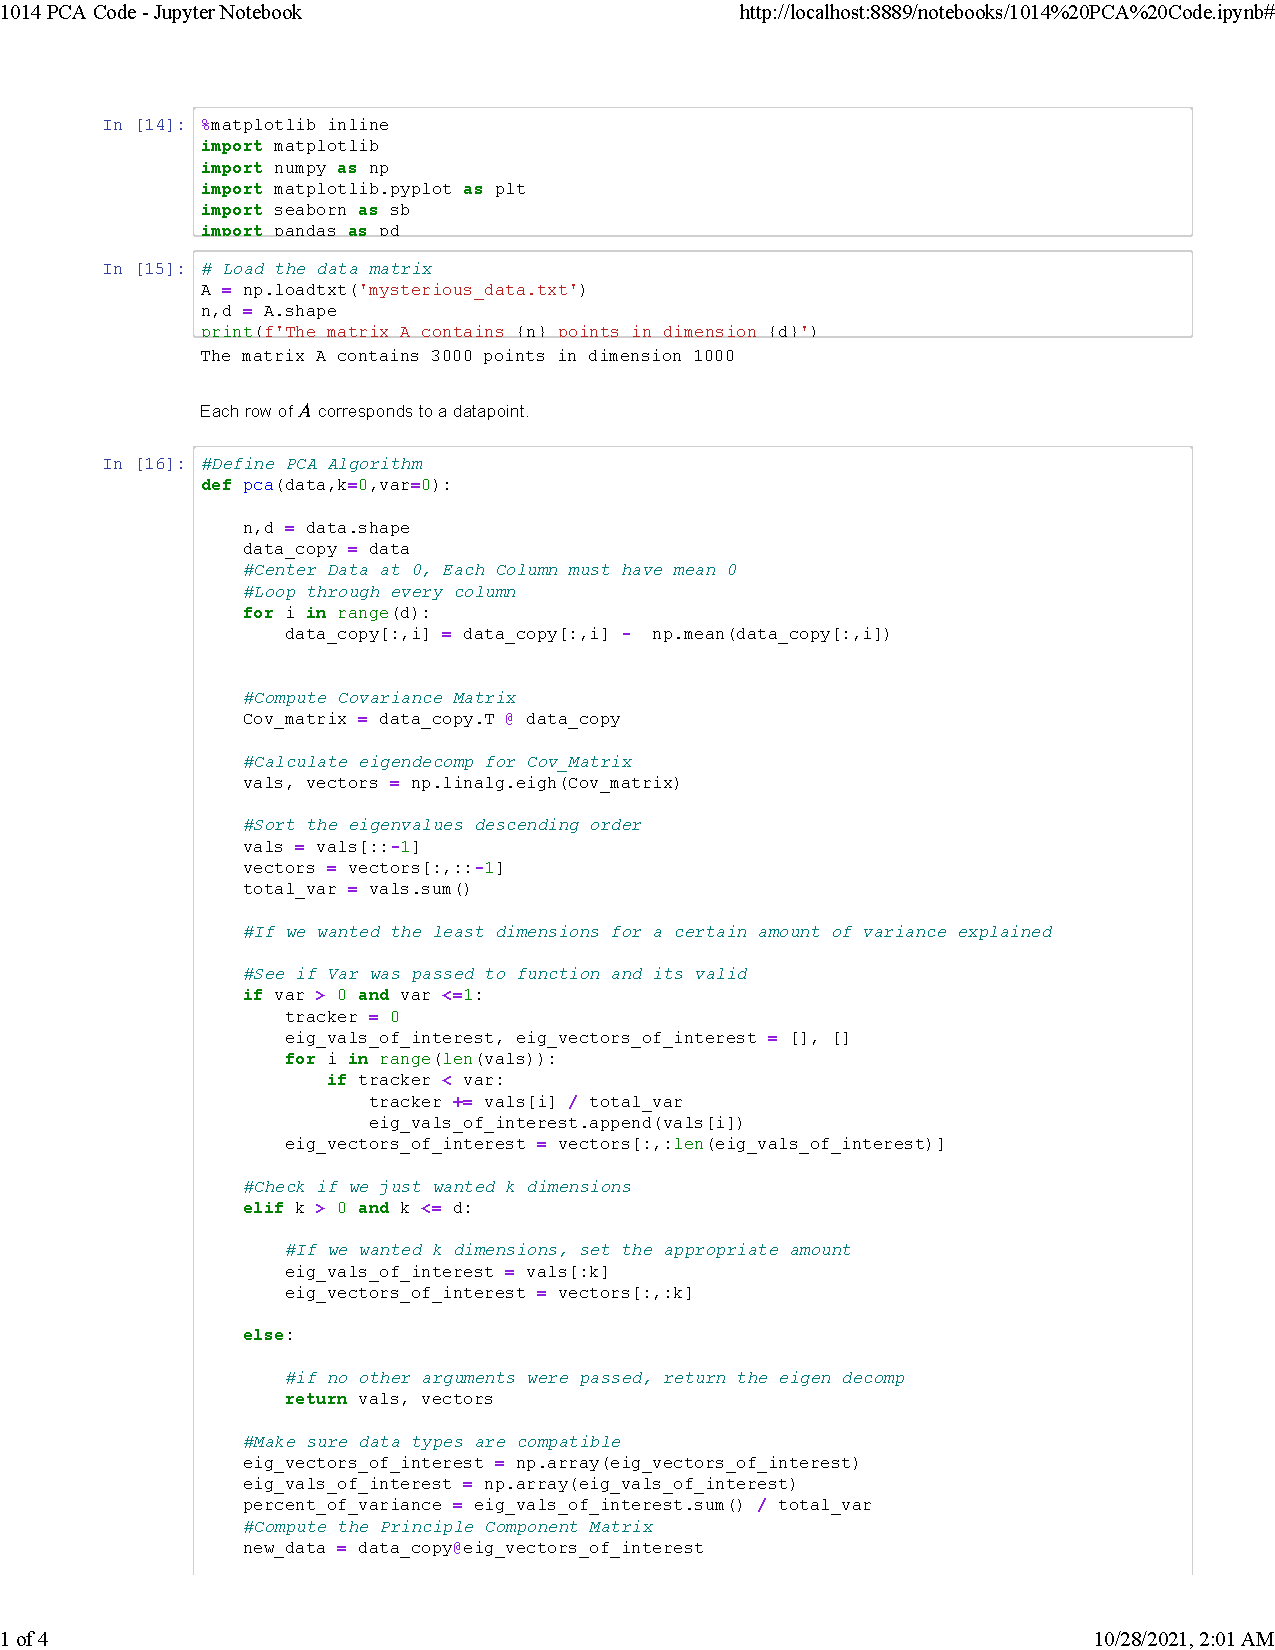
\includepdf[pages=-]{1014 PCA Code - Jupyter Notebook.pdf}


\vspace{5mm}

\section{Problem 7.4}
	Let $A \in \mathbb{R}^{n \times n}$ be a symmetric positive semi-definite matrix. Prove that there exists $B \in \mathbb{R}^{n \times n}$ positive  semi-definite such that $A = B^2$.\\

Since we know that A is positive semi definite, we know that it has eigenvalues of at least 0. Therefore, we can take the square root of the eigenvalues. We also know that A is square symmetric, and therefore Since $A$ is square symmetric, we know $A^k=PD^kP^T$, where D is the diagonal matrix of A's eigenvalues, and P, and $P^T$ are the orthonormal basis of A's eigenvectors.

$$
\text{Let } D = \begin{pmatrix}
\lambda_1 & \dots &  0_{1,n}\\
0 & \ddots & 0 \\
0_{n,1} & \dots & \lambda_n
\end{pmatrix} \text{ and therefore let }D^{\frac{1}{2}} = \begin{pmatrix}
\sqrt{\lambda_1} & \dots &  0_{1,n}\\
0 & \ddots & 0 \\
0_{n,1} & \dots & \sqrt{\lambda_n}
\end{pmatrix}
$$ 
And therefore, let $B=PD^{\frac{1}{2}}P^T$. 

\begin{equation}
    \begin{split}
        A &= PDP^T \\
        PDP^T &= PD^{\frac{1}{2}}P^TPD^{\frac{1}{2}}P^T\\
        PDP^T &= BB\\
        A &= B^2 \qed
    \end{split}
\end{equation}

Since A is positive semi definite, B must also be positive semi definite, as the eigenvalues of A are greater or equal to 0, and the eigenvalues of $B$ are equal to the square root of the eigenvalues of $A$, which of course will be positive.

% \centerline{\pgfornament[width=7cm]{87}}

%\bibliographystyle{plain}
%\bibliography{./references.bib}
\end{document}